\documentclass[a4paper,12pt]{article} 

%%% Работа с русским языком
\usepackage{cmap}                           % поиск в PDF
\usepackage{mathtext} 			 	       % русские буквы в формулах
\usepackage[T2A]{fontenc}               % кодировка
\usepackage[utf8]{inputenc}              % кодировка исходного текста
\usepackage[english,russian]{babel}  % локализация и переносы
\usepackage[left=2cm,right=2cm,
    top=2cm,bottom=3cm,bindingoffset=0cm]{geometry}
\usepackage{wrapfig}
\usepackage{gensymb}
\usepackage{textcomp}
\usepackage{multirow}
\usepackage{pgfplots}
\usepackage{amsmath,amsfonts,amssymb,amsthm,mathtools} % AMS
\usepackage{euscript}	 % Шрифт Евклид
\usepackage{mathrsfs} % Красивый матшрифт
\usepackage{graphicx}%Вставка картинок правильная
\usepackage{float}%"Плавающие" картинки
\usepackage{wrapfig}%Обтекание фигур (таблиц, картинок и прочего)
\title{Лабораторная работа 8.1

Тепловое излучение}
\author{Кагарманов Радмир Б01-102}
\date{9 октября 2023 г.}

\begin{document}
\maketitle
\thispagestyle{empty}
\newpage
\setcounter{page}{1}

\paragraph{Цель работы:} определить постоянные Планка и Стефана-Больцмана.

\paragraph{В работе используется:} пирометр с исчезающей нитью, модель АЧТ, трубка с кольцами, лампа накаливания, неоновая лампочка, амперметр, вольтметр.

\paragraph{Теория\\}
Для измерения температуры разогретых тел, удалённых от наблюдателя, применяют методы оптической пирометрии, основанные на использовании зависимости испускательной способности исследуемого тела от температуры.\par
Оптический пирометр представляет собой зрительную трубу, внутри которой имеется накаливаемая нить. При совпадении яркостей нить перестаёт быть видимой на фоне изображения раскалённого тела.

\begin{figure}[!h]
\centering
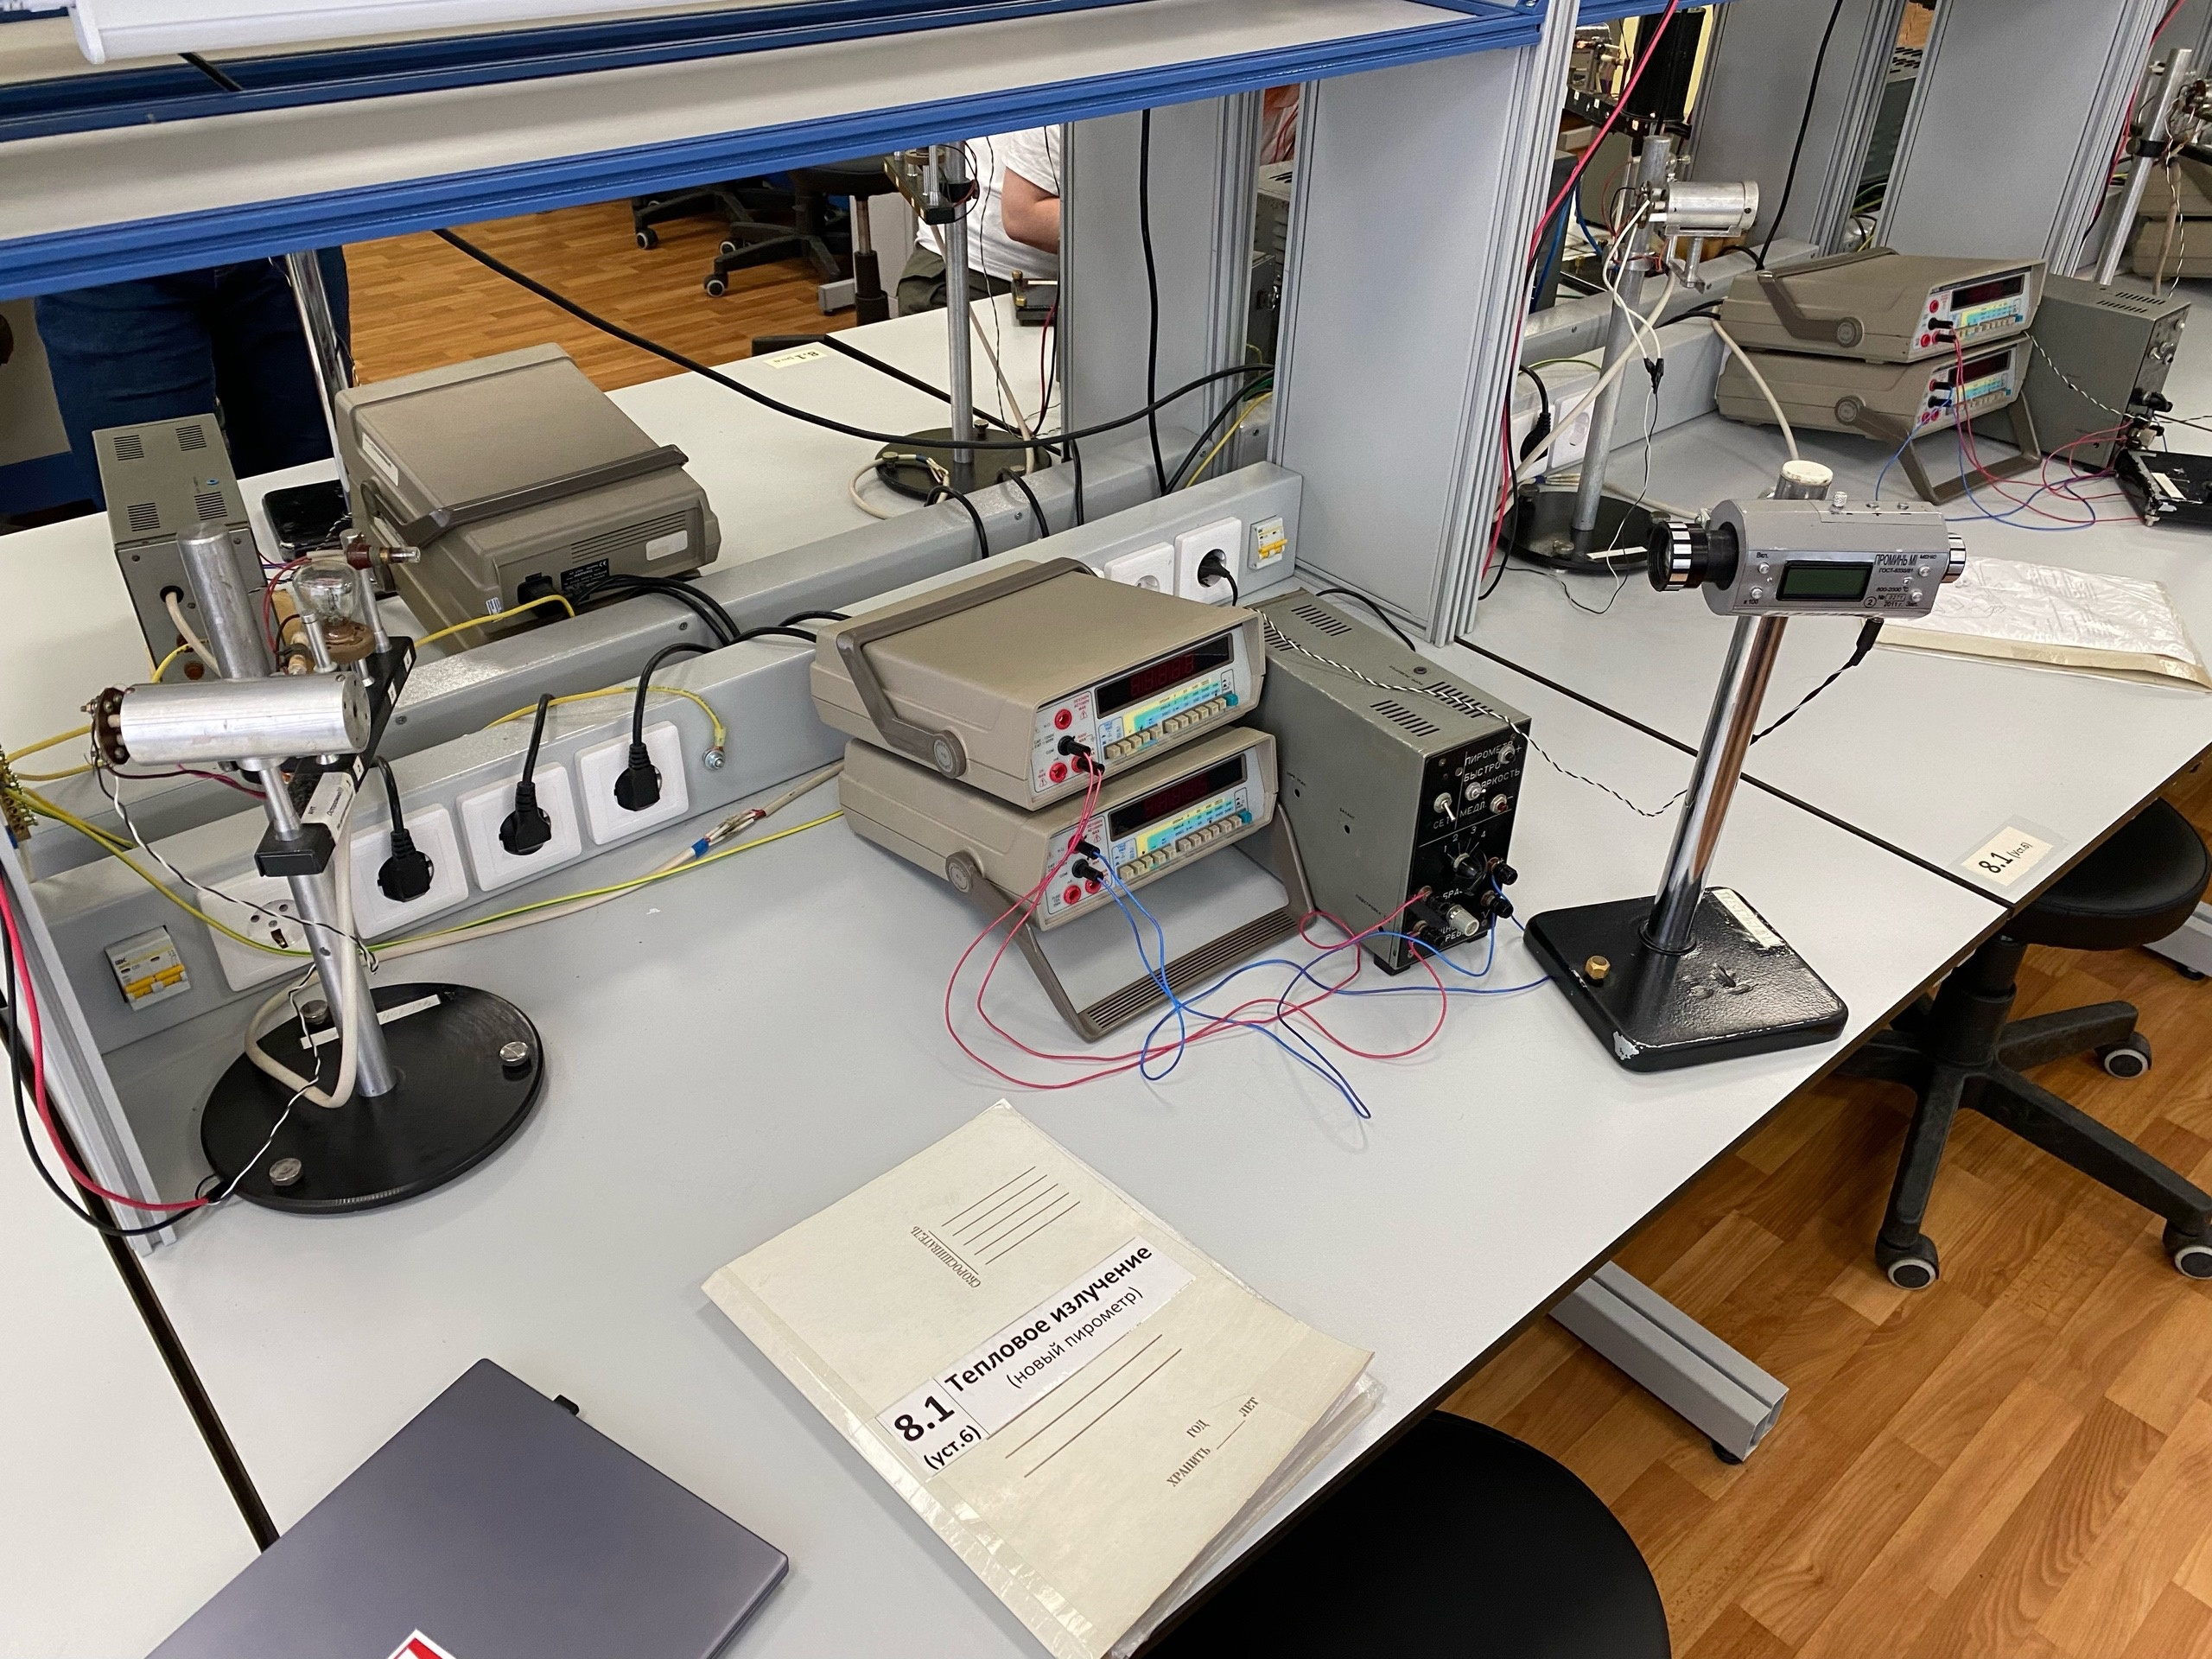
\includegraphics[width=0.8\linewidth]{-5C9LfcpZBk.jpg}
\caption{Экспериментальная установка}
\label{fig:mpr}
\end{figure}

\paragraph{Обработка результатов}
\subparagraph{1.} Построим график зависимости $ln~W=ln~(\varepsilon_T)+nln~T$ и определим $n$. $W$ найдём с помощью амперметра и вольтметра. $n=3,26$.

\begin{figure}[!h]
\centering

\includegraphics[width=1\linewidth]{graph1.png}
\caption{График зависимости $ln~W=ln~(\varepsilon_T)+nln~T$.}
\label{fig:mpr}
\end{figure}


\subparagraph{2.} Найдём величину постоянной Стефана-Больцмана по формуле:

\begin{equation}
    \sigma = \frac{W}{\varepsilon_T S T^4},
\end{equation}
где $S=0,36см^2$, а $\varepsilon_T$ можно посмотреть в таблице.
\begin{center}
    $\sigma = 45,9\cdot 10^{-12}\frac{Вт}{м^2K^4}, ~ T = 1773~K$\\
    $\sigma = 40,9\cdot 10^{-12}\frac{Вт}{м^2K^4}, ~ T = 1873~K$\\
    $\sigma = 40,8\cdot 10^{-12}\frac{Вт}{м^2K^4}, ~ T = 1973~K$
\end{center}
\subparagraph{3.}Из найденных значений $\sigma$ определим постоянную Планка по формуле:
\begin{equation}
    h = \sqrt[3]{\frac{2\pi^5k_{Б}^4}{15c^2\sigma}}
\end{equation}

\begin{center}
    $h = 7\cdot 10^{-34}~Дж\cdot c$\\
    $h = 3,4\cdot 10^{-34}~Дж\cdot c$\\
    $h = 3,4\cdot 10^{-34}~Дж\cdot c$
\end{center}
\paragraph{Вывод:} в данной лабораторной работе мы определили постоянные Стефана-Больцмана и Планка.

\end{document}
